\subsection{Regulador L79XX}
Además de los reguladores anteriormente mencionados, también existen reguladores
de tipo negativo que proveen una salida de voltaje inverso.

En la \textbf{figura~\ref{circuito10}} se muestra un circuito regulador
\textbf{L7909CV} que fija el voltaje a $-9[\text{V}]$ filtrado por un capacitor
de $470[\mu\text{F}]$ en la entrada y un capacitor de $10[\mu\text{F}]$ para la
salida.

\begin{figure}[!h]
\centering
\includegraphics[scale=1.1]{diagramas/10.regulador2.eps}
\caption{Regulación de voltaje con \textbf{L7909CV}.}
\label{circuito10}
\end{figure}

\subsubsection{Simulación}
Se utilizó el software \emph{Quite Universal Circuit Simulator.} versión 23.3.1
para la simulación de la regulación de voltaje con el circuito integrado
\textbf{L7909CV} este puede verse en la \textbf{figura~\ref{simulacion10}}.

\begin{figure}[!h]
\centering
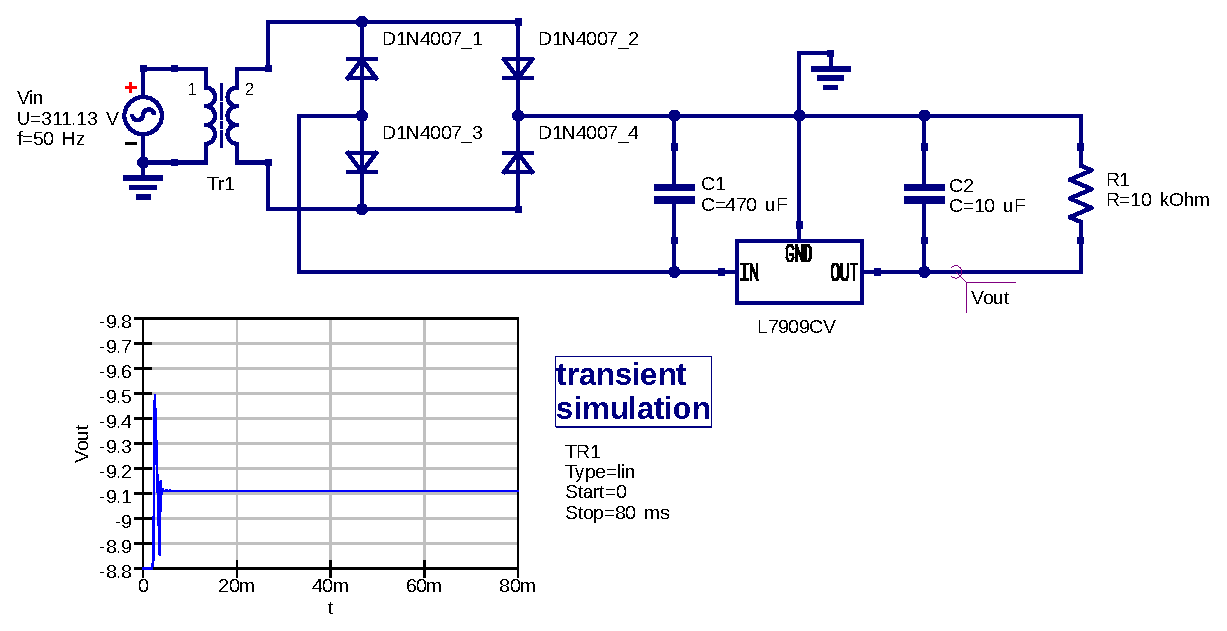
\includegraphics[scale=0.75]{simulacion/10.regulador2.eps}
\caption{Simulación del regulador \textbf{L7909CV}.}
\label{simulacion10}
\end{figure}

\begin{figure}[!h]
\centering
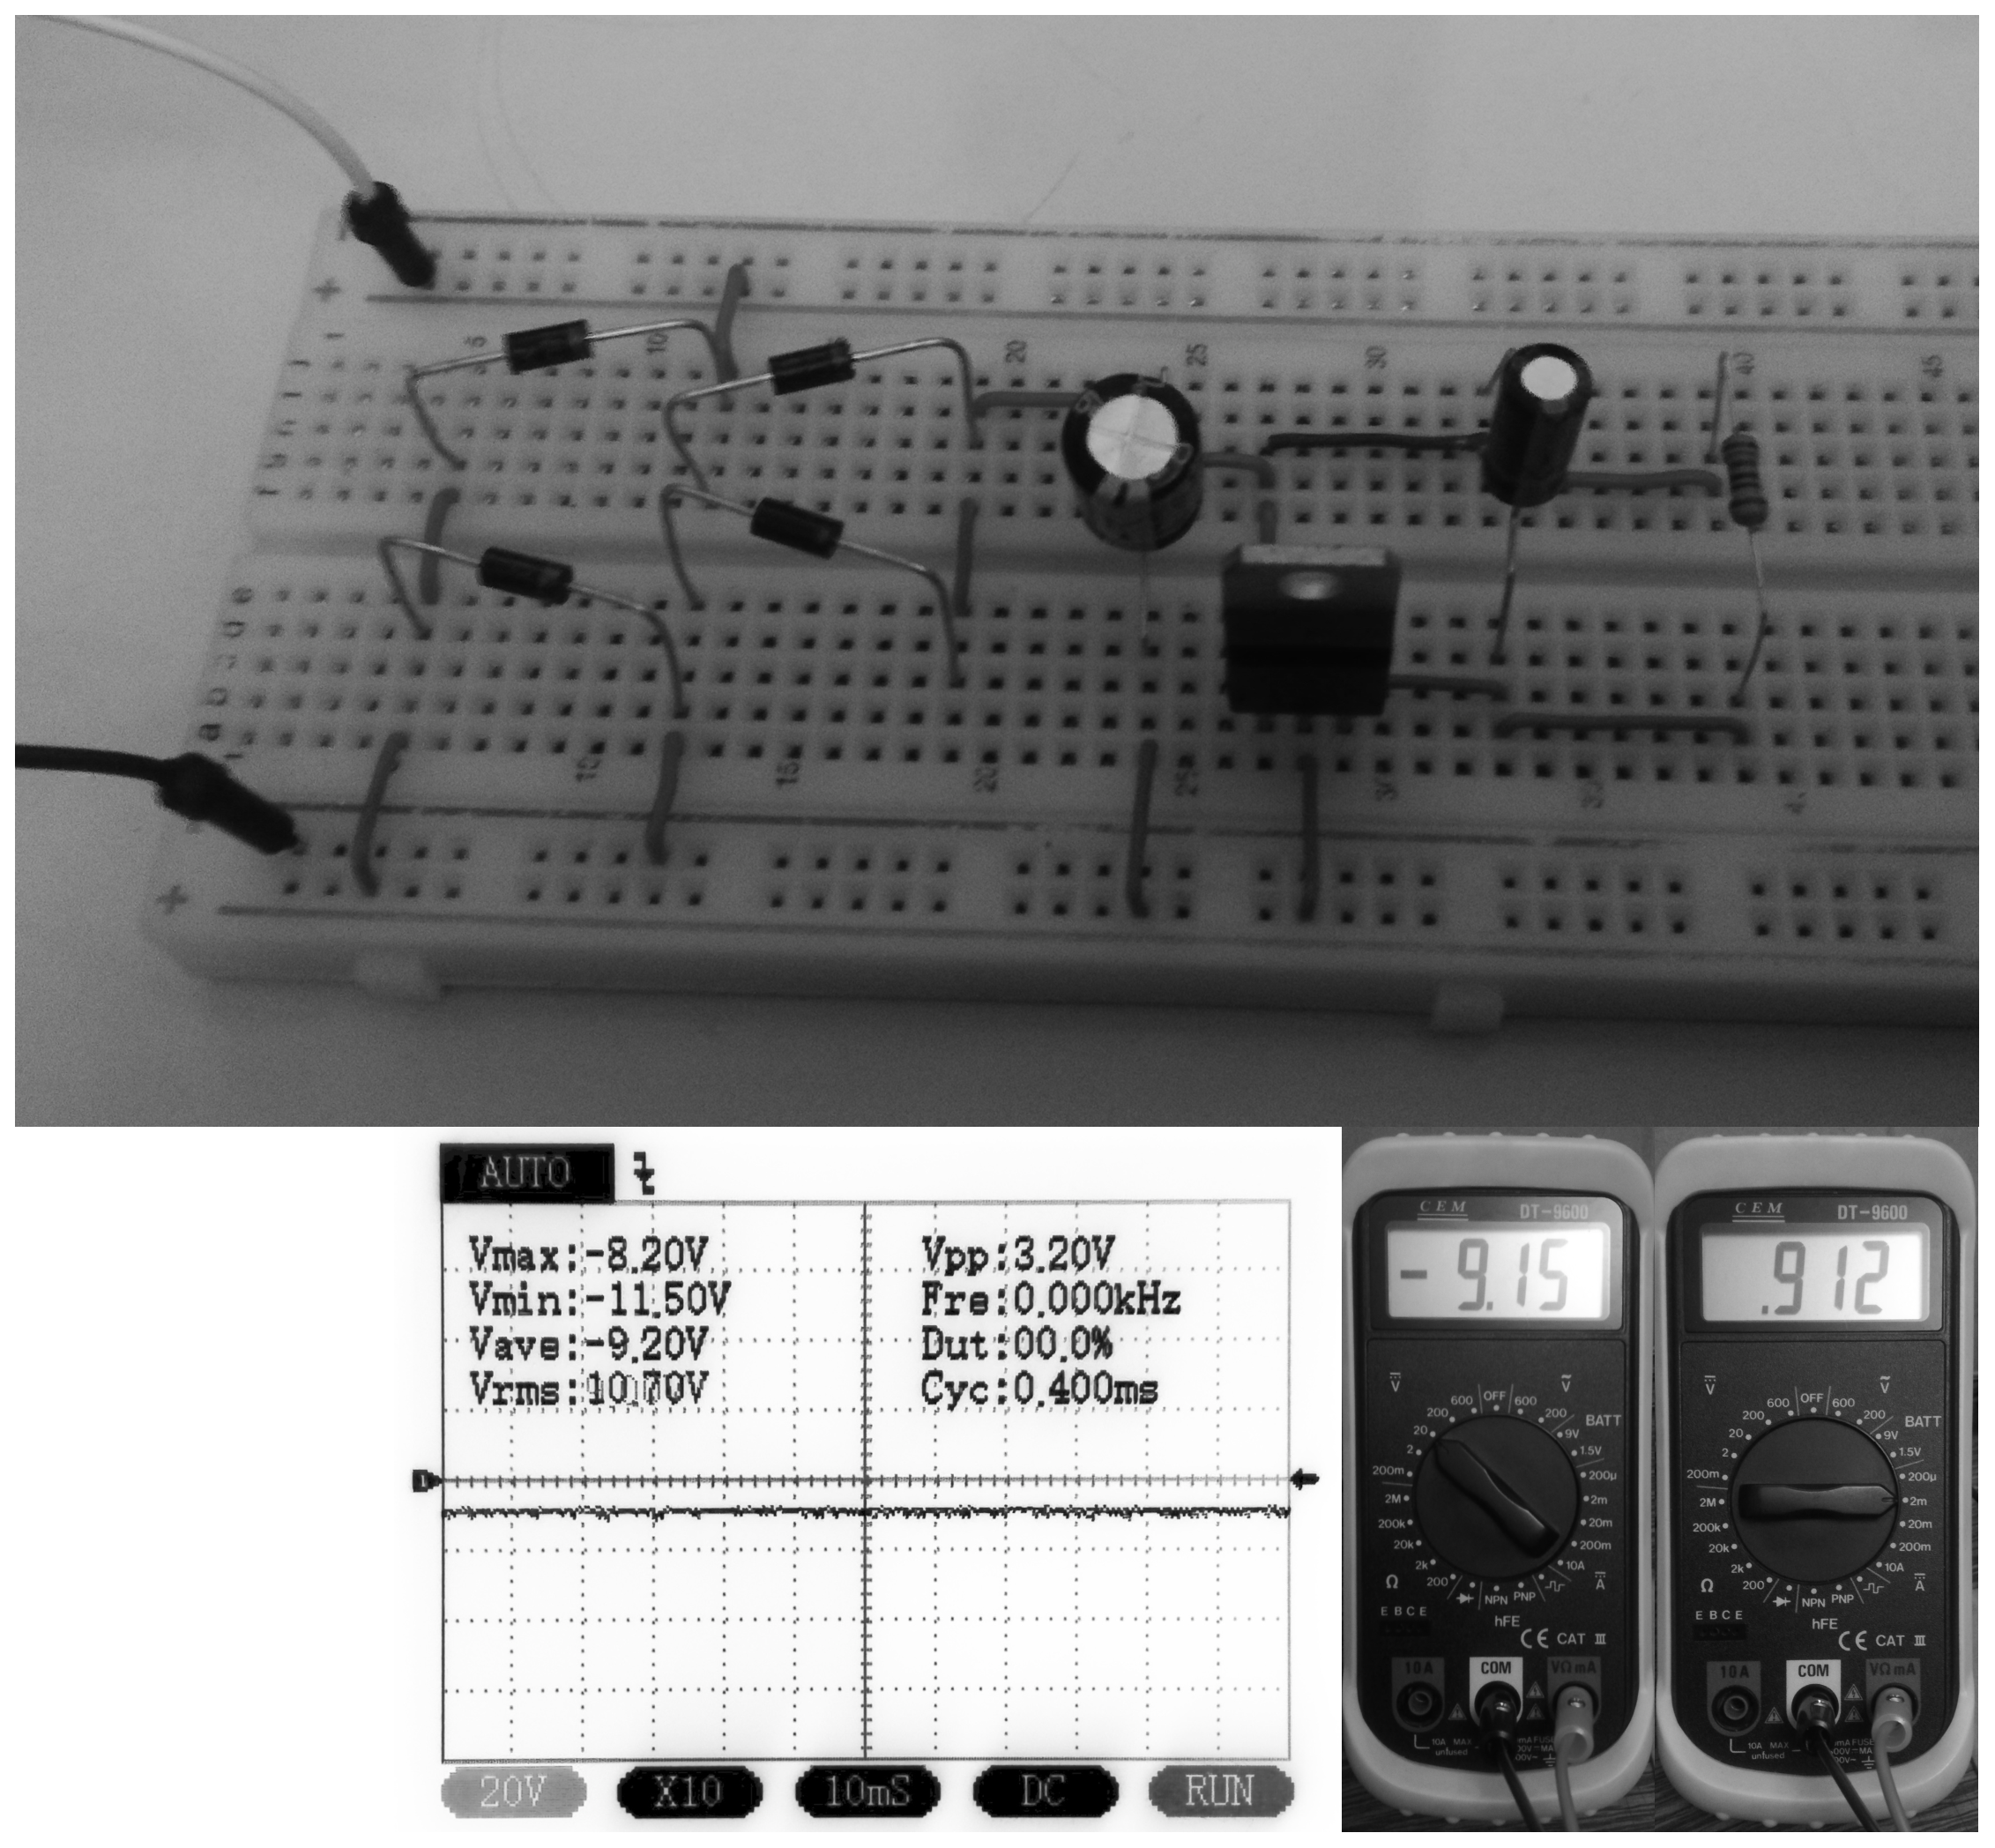
\includegraphics[scale=0.26]{fotos/10.regulador2.eps}
\caption{Regulador \textbf{L7909CV}, salida del osciloscopio\\
y medición de voltaje y corriente.}
\label{laboratorio12}
\end{figure}

\subsubsection{Laboratorio}
Se presenta el regulador \textbf{L7909CV} armado en laboratorio, su señal de
voltaje de salida en osciloscopio, así como su voltaje y corriente en un
multímetro para una resistencia de carga de $10[\text{k}\Omega]$ en la
\textbf{figura~\ref{laboratorio12}}.

